\chapter{\IfLanguageName{dutch}{Stand van zaken}{State of the art}}%
\label{ch:stand-van-zaken}

% Tip: Begin elk hoofdstuk met een paragraaf inleiding die beschrijft hoe
% dit hoofdstuk past binnen het geheel van de bachelorproef. Geef in het
% bijzonder aan wat de link is met het vorige en volgende hoofdstuk.

% Pas na deze inleidende paragraaf komt de eerste sectiehoofding.

The research towards skill-recognition will be done in several steps.
The first step involves examining challenges of judging and recent adaptations for judging routines.
Next follows a brief overview of DD3-skills, to further specify and clarify the DD3 components.
Skills, combinations and transitions will than be mapped in a skill-matrix, nearing close to binary computer output.
Upon specifying these components, it is revealed that their are certain challenges for AI models in order to recognize these skills.
Something is needed that can use video information to localize the jumper, sequence the video, and recognize the performed skill.
These three main requirements are elaborated in computer vision literature. % TODO : ask alongside previous insights, is that NextJump?
Finally some challenges remain such as group activity or unknown/unusual skills.

% I think it would be good to slightly restructure your literature review for
%  reasons of clarity and to provide more detail on certain topics.

% Perhaps something like: challenges of judging + recent adaptations to
%  address these > detailed description of skills and skill combinations
%   (skills matrix) > summarizing paragraph highlighting
%    the particular challenges for AI models: you need something
%     that can use video information to localize the jumper,
%      sequence the video, and recognise the performed skill
%      > investigation into existing technologies that seem
%       promising for your use case (computer vision, HAR,
%        jumper localization, video segmentation,
%        then insights from previous use of tech to recognize skills)
% > remaining challenges (group activity + unknown/unusual skills)

\section{Challenges of judging}
\label{subsubsec:bp-literature-judge-challenges}

\begin{table*}[]
    \begin{tabular}{lllllllll}
        Year & World & Europe & Belgium & Usa   & Hungary & Germany & China \\ \hline
        1998 &       &        &         &       &         &         &       \\
        1999 & 80    &        & 80      &       &         &         &       \\
        2012 &       &        &         &       &         &         &       \\
        2015 &       &        &         &       &         &         &       \\
        2016 & 111   & 103    &         &       &         & 103     &       \\
        2019 & 111   &        & 102     & 105.5 &         &         &       \\
        2020 & 111   &        & 102     & 105.5 &         &         &       \\
        2021 & 111   &        & 103.5   & 105.5 &         &         &       \\
        2022 & 111   &        & 103.5   & 105.5 &         &         &       \\
        2023 & 113   &        & 103.5   & 106   &         &         & 113   \\
        2024 & 113   & 108    & 103.5   & 106   &         &         & 113
    \end{tabular}
    \caption[speed records males]{History of speed records males, \autocite{www_speed_30s_1999_WORLD}, \autocite{www_speed_30s_2024_BE}, \autocite{www_speed_30s_2024_IJRU_WORLD}, \autocite{www_speed_30s_2024_USA_AMJRF}}
    \label{tbl:speed-records-history-male}
\end{table*}

\begin{table*}[]
    \begin{tabular}{lllllllll}
        Year & World & Europe & Belgium & Usa   & Hungary & Germany & China \\ \hline
        1998 & 83    &        &         &       & 83      &         &       \\
        1999 &       &        &         &       &         &         &       \\
        2012 &       &        & 102     &       &         &         &       \\
        2015 & 105   & 105    &         &       & 105     &         &       \\
        2016 & 105   & 105    & 102     &       & 105     &         &       \\
        2019 & 108.5 & 105    & 102     & 100.5 & 105     &         & 108.5 \\
        2020 & 108.5 & 105    & 102     & 100.5 & 105     &         & 108.5 \\
        2021 & 108.5 & 105    & 102     & 100.5 & 105     &         & 108.5 \\
        2022 & 108.5 & 105    & 102     & 100.5 & 105     &         & 108.5 \\
        2023 & 108.5 & 105    & 102     & 100.5 & 105     &         & 108.5 \\
        2024 & 108.5 & 105    & 102     & 100.5 & 105     &         & 108.5
    \end{tabular}
    \caption[speed records females]{History of speed records females, \autocite{www_speed_30s_1999_WORLD}, \autocite{www_speed_30s_2024_BE}, \autocite{www_speed_30s_2024_IJRU_WORLD}, \autocite{www_speed_30s_2024_USA_AMJRF}}
    \label{tbl:speed-records-history-female}
\end{table*}

As introduced earlier, based on own experiences and statements of colleagues, the sport is evolving. These statements are supported by fellow athletes, or commentary from the IJRU world championship livestream day 1 \autocite{IJRU_yt_2023_livestream_day1} to day 8 \autocite{IJRU_yt_2023_livestream_day8}.
Speed records are slowly rising, see tables \ref{tbl:speed-records-history-male} or \ref{tbl:speed-records-history-female} \footnote{\autocite{www_speed_30s_1999_WORLD}, \autocite{www_speed_30s_2024_BE}, \autocite{www_speed_30s_2024_IJRU_WORLD}, \autocite{www_speed_30s_2024_USA_AMJRF}}, also quads or quints in single rope freestyles are becoming the norm, where 10 to 15 years ago, it was considered a wow factor. This is also the case for double dutch; more variations, more turner involvements, faster and longer skill-sequences etc.
The evolution of the sport requires an update of the evaluation of it. And indeed over the past few years, a few changes have been implemented to address some of the challenges the rising complexity of routines poses for human AI judges, such as splitting responsibility, multiple judging panels, the adaptation of rules or allowing post-review.

\subsection{Splitting responsibility}
With the current rules, 11 judges, supervised by a head judge, are divided in two main categories. Three of them watch and annotate how difficult a routine is. The other 8 judge the creativity of the routine. Creativity is further split into execution, entertainment, musicality and variation, each judged by two jurors \footnote{In case there are insufficient judges, some positions remain vacant}. This breakdown allows increased attention on different aspects of a routine, thus decreasing potential observation mistakes.

\subsection{Multiple panels}
Using two or more judge-panels, more freestyles can be evaluated at the same time. While one panel is watching a freestyle, the other can summarize and calculate the total score of the previous routine. Panels and routines are often arranged to judge the same category, e.g. juniors vs seniors, which decreases the effect of human differences between judges, such as how strict one is when evaluating, incorrect memorization of skill levels, fatigue, ...

\subsection{Adapting the rules}
In order to account for rising difficulty levels, variation, new skills, simplified judging, ... rule guidelines change. This can impact the way freestyles are evaluated, in ways of thinking, memorizing or calculating the level, score or deduction of a skill. One such example are the current rules for Double Dutch freestyles which uses 'snapshot' principle, which is a way of judging where you calculate a skill level right after a jumper has performed a skill, as if you take a picture. However, multiple rotations of the rope aren't 'visible' in a single imaginary image/snapshot. In other words, a snapshot is a small time interval incorporating multiple different aspects for a judge to take notice of. Using this principle requires a lot of thinking during the routine, requiring the post-review, to correctly assign difficulty levels to skill-combinations. These rules where applied during the seasons 23'-24' and 24'-25' and will be changed again.

\subsection{Review at slower speed}
In recent years, the video replay was introduced on high-level competitions \footnote{High-level competitions contain world championships or local finals (e.g. Belgium)} to review a double dutch freestyle at slower speed to accurately assign the performed skill-level.
Even in slow motion, differences between assigned scores of judges exist when calculating the total level of skill, transition, turners and rotational speed.

\subsection{Challenges summary}
Incorporating all these things brought jump rope to where it is. To increase the accuracy of difficulty score assignments, we try to find improvements. One of these is exploring automatic skill-recognition by using AI. When skills are recognizable by a program, they can be mapped to their corresponding level, contributing towards the end score. Knowing what's represented in an image or a video is called computer vision. % TODO : source

\section{Jump rope skills introduction}
\label{subsec:bp-literature-basisskills}

Earlier we described the presence of multiple disciplines in jump rope. One particular discipline within jump rope that is highly complex and therefore challenging in terms of difficulty scoring is a Double Dutch Single Freestyle (DD3). This study will focus on this type of freestyle to explore how and in what way recent advancements in machine learning can facilitate and improve difficulty scoring.

% \subsection{Double Dutch Single Freestyle - DD3}
% \label{subsubsec:literature-dd3}
\medskip

% TODO : add DD figure for clarification
DD3 consists of two turners and one jumper alternating ropes. Elements in double dutch are similar to single rope, but different at the same time. The jumper can execute skills, mainly powers \footnote{powers/strength type skills}, gymnastics or footwork. Meanwhile, turners can manipulate the rope by rotating multiple ropes underneath the athlete in a single jump, called multiple unders. Another turner involvement could be turner-skills, which are restrictions like crossing the arms, restricting one of your arms behind your back (EB), maybe both arms (TS) or under your leg. Turners can even perform footwork, powers or gymnastics themselves. \footnote{Footwork as a turner doesn't raise your score.}
To judge double dutch, `snapshots` are taken, then the corresponding level is given depending on the combination of turners, skills and rope-rotations.

Like any discipline, mistakes can happen for which points are deducted from the total score.

The following examples illustrate how scores are assigned for DD3 routines. Levels are only given when the jumper is performing a skill, these can be raised by turner involvements or skill modifiers.

% TODO : bijlage bij BP?
\begin{itemize}
    \item Powers
    \begin{itemize}
        \item push-up - (= plank position - lvl 2)
        \item split (2)
        \item frog - (= handstand) (2)
        \item swift/V-kick (3)
    \end{itemize}
    \item Gymnastics
    \begin{itemize}
        \item cartwheel (2)
        \item kip (3)
        \item salto (4)
    \end{itemize}
    \item Turners
    \begin{itemize}
        \item cross (c - crossed arms on the stomach) (+2/+0)
        \item crouger (raise left knee, put left your arm underneath it from the inside to the outside) (+1)
        \item EB (arm on stomach + arm on back) (+1)
        \item TS (arms crossed behind the back) (+1/+1)
    \end{itemize}
    \item Multiples
    \begin{itemize}
        \item double - DU - 2 rotations (+1)
        \item triple - TU - 3 rotations (+2)
        \item quad - QU - 4 rotations (+2)
        \item quint - 5 rotations (+3)
    \end{itemize}
    \item Modifiers
    \begin{itemize}
        \item using one hand (+1 or +0 depending on the skill)
        \item pushing of 2 feet (+1 or +0 depending on the skill)
        \item turntable - (+1 for each quarter rotation for a transition between the same power. e.g. push-up turntable = push-up to push-up with a quarter turn)
    \end{itemize}
\end{itemize}

While these additions may seem simple, the combination of not knowing what will performed next, while keeping an eye on three people executing skills sequentially in about two thirds of a second makes it hard to evaluate for judges.

\section{Skill-matrix - complexity \& levels - towards model accuracy}
\label{subsec:skillcomplexiteit}

\begin{figure}
    \centering
    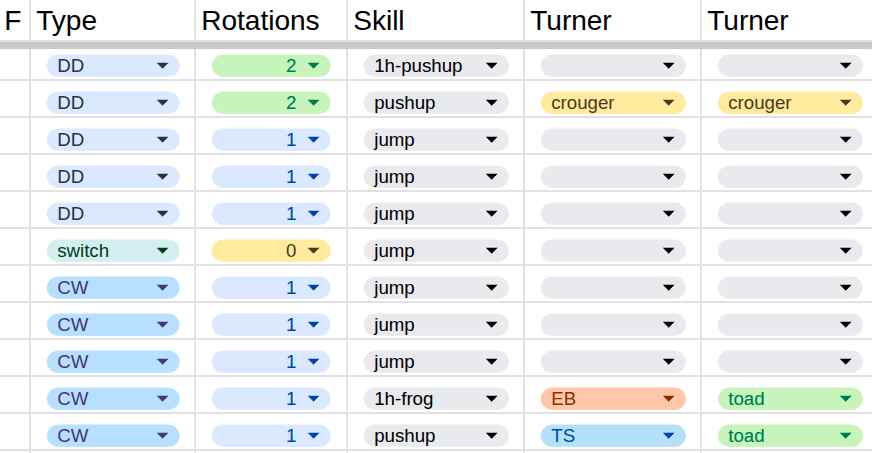
\includegraphics[width=0.95\linewidth]{img/doubledutch-matrix}
    \caption[skill-matrix-DD]{First draft representing a skill-matrix used for Doube Dutch.}
    \label{fig:doubledutch-skill-matrix}
\end{figure}

The previous section, (\ref{subsec:bp-literature-basisskills}), provides a basic explanation of the skills to be judged, along some examples. To be able to develop a model that can accurately recognize all skills, it is necessary to draw up a detailed skills matrix. This section explains the composition of the skill-matrix, in order to give a better understanding on the total accuracy of the models later on. As described earlier, skills come with many transitions, take the first skill-matrix representation in figure \ref{fig:doubledutch-skill-matrix} to better understand skills and transitions.

\textbf{Type:} You have four styles of turning in double dutch; the normal way or double dutch (DD), reversing the rope rotation, sort of like backwards called irish dutch (irish), the chinese way of turning, chinese wheel (CW) or only using one rope or the two combined as a single rope, called single dutch or one rope.

\textbf{Rotations:} The amount of ropes passing underneath the athlete in one jump.

\textbf{Turner:} There are two turners, so two columns, where each turner can execute a turner involvement. Examples are EB, toad or crouger. The cross is in most cases performed by both turners, otherwise the ropes are tangled.

\textbf{Skills:} Mostly powers or gymnastics, but could also be footwork \footnote{Footwork will not be further specified in this paper}. Further distinction or organizing can happen as variation and transitions of powers and gymnastics exists. A recap of different skills would be: pushups, splits, crabs, frogs, swift, cartwheel, salto, webster, suicide, handsprings, round offs \dots % TODO : refer pictures, examples of skills in attachment.
Depending on the exact power or gymnastic, certain characteristics or transitions could be applied:

\begin{itemize}
    \item one handed
    \item one or two feet push-off (e.g. frog vs high frog, salto vs webster, suicide one vs two legged push-off)
    \item turntable \footnote{On way of turning your bodyposition, can be done per quarter e.g. quarter turntable push-up}
    \item full body rotation \footnote{Other way of turning your body, requires full turns}
    \item consecutive \footnote{Consecutive handstands are considered harder and thus get you extra points, not the case with push-up}, e.g. frog after frog
\end{itemize}

Applying these transitions, characteristics allows for even more variation, which will increase the number of awarded points. Repeated skills does not lead to. Repetitions are only defined by the skills in the ropes, the speed of the rope (rotations) and the type of turning \footnote{No difference will be made between irish turning and double dutch. Also, only the first skill in single dutch counts}.

\medskip

The skill-matrix is subject to change over time. For the initial research and PoC, skills may be simplified or left out of the matrix will be left out for the PoC. Other than skills, jumpers and turners can switch positions, which is called a transition. These transitions do not fit in the matrix discussed below and are also omitted in the PoC.
Each column in the first skill-matrix-example \ref{fig:doubledutch-skill-matrix} can only contain one property, for which softmax can be used, while between multiple columns, no relation is required and meaning the skills can be predicted separately. This can be solved using a multi-branch output as described in by \textcite{Coulibaly_2022}. This can result in a guessed skill being partially correct, e.g. turner correct, but wrong rotational amount.




On another note, \textcite{Guo_2017} explain that softmax isn't always a good indicator of confidence. They mention that when a model has good calibration, the accuracy should align with the confidence of the prediction. E.g. when you predict a skill has an 80\% chance being of being a push-up, then this prediction or 80\% of the predicted push-ups should be correct. Predictions using softmax tend to be overconfident.



\section{Computer vision}
\label{subsec:bp-literature-computer-vision}

\begin{table*}[t]
    \centering
    \begin{tabular}{|l|l|l|}
        \hline
        & SR & DD3 \\ \hline
        \#Freestyles & 500-1000+ & 286-352 \\ \hline
        Hours & 8h-16h+ & 5-6h \\ \hline
        MVP & basic skill recognition & basic powers, gyms, turnerskills \\ \hline
        Level-guessing & 0 to 8 & 0 to 6/8 \\ \hline
        Theoretical level limit & 8+ levels possible & 8+ levels possible \\ \hline
        skill-matrix & finer hand movements & larger actions compared to SR \\ \hline
        individuals & 1 & 3 \\ \hline
    \end{tabular}
    \caption[Collected videos data comparison]{Data comparison between single rope freestyles and double dutch single freestyles. The number of freestyles is an estimation of the available and potential extra recordings possible on competitions during the research process.}
    \label{tbl:data-comparison-sr-dd}
\end{table*}

% TODO : footnote refer to table above for numeric data
To automatically recognize skills, input data is needed. There are quite some videos on socials, as well as in-house recordings, see table \ref{tbl:data-comparison-sr-dd}, so the choice to learn from videos was made quickly. This is also the choice for NextJump, a speed counter, counting how many speed-steps there are within a given time span.
Computer vision is the field of study in which computers recognize features, people or other objects in digital imagery. More specifically, the focus is recognizing human actions in these recordings, called Human Activity Recognition or HAR \autocite{Pareek_2020}.


Other papers mention slight adaptations to human action recognition, namely Human Gait Recognition, HGR, or Human Pose Estimation, HPE. Although the three techniques are closely related, each of them has a different nuance. Gait recognition looks at a person's typical movements, gestures or behavioral patterns \autocite{Alharthi_2019}, while pose estimation looks specifically at poses or special expressions \autocite{Song_2021}. They also talk about how pose recognition, e.g. skeleton-based, can be used as a tool to improve activity labeling.
While these are interesting techniques, more effort is put into action recognition.





\subsection{Computer vision in other sports}
\label{subsubsec:bp-literature-computer-vision-sports}

\textcite{Soomro_2014} published a book about the first advancements in computer vision since it was applied to sports. In addition, \textcite{Yin_2024} published a paper on the latest advancements of computer vision in teams competitions. Although relatively popular, neither of them really talks about gymnastics, which is closer related to jump rope than sports like tennis, basketball or cricket.
Given examples by those two sources of performed computer vision tasks are: player tracking, following the ball trajectory (e.g. in cricket, football, tennis), human to human interaction (e.g basket) or detecting action types (e.g. running, walking, hitting the ball) or predicting the sport itself. (e.g. Olympics dataset).
% ------------------------
% Jump rope related sports
% ------------------------

A successful example recognizing static images on gymnastics rings, \textcite{Abdullah_2023}, illustrates the possibility of recognizing the main body positions in double dutch freestyles. Although the dataset is fully balanced and with a limited amount of classes, extending it shouldn't pose an issue. Preferably, identifying skills should incorporate the time aspect.
\textcite{Zahan_2023} modified the Long Short Term Memory model (LSTM-model) to incorporate longer time sequences, to predict a full score of a routine which is static and not future proof. Changes in rules would make older scores useless and request for mistakes.

Meanwhile, the International Gymnastic Federation (\href{https://www.gymnastics.sport/site/}{FIG}) has been working with Fujitsu sinds 2017 in order to create a \href{https://www.fujitsu.com/global/themes/data-driven/judging-support-system/}{Judging Support System}. Initially, sensor data was used in order to predict skills, however in their official launch, \autocite{Fujitsu2023launch}, they mentioned a transition towards camera based image analysis, reaching higher performance. Which model they use is unknown.
Combining these examples and earlier research, a robust action recognition model can be developed detecting key aspects of a a video. These aspects, such as the number of hands, feet, body rotations and the main pose/action, can then be mapped with a level/score resulting in the full difficulty score of a routine.

\subsection{NextJump Speedcounter}
\label{subsubsec:bp-literature-nextjump-speedcounter}

% \begin{figure}
%     \centering
%     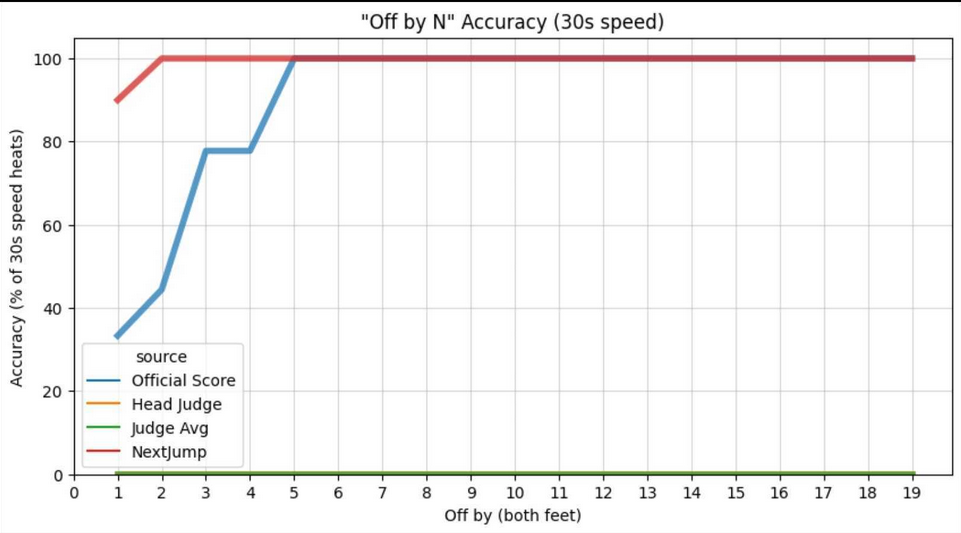
\includegraphics[width=0.95\linewidth]{img/nextjump-off-by-feet}
%     \caption[nextjump-results]{Comparison of avg scores given to a jumper, compared to the effective score. Results are from 2024 AMJRF nationals.}
%     \label{fig:nextjump-results-off-by-feet}
% \end{figure}

\begin{figure}
    \centering
    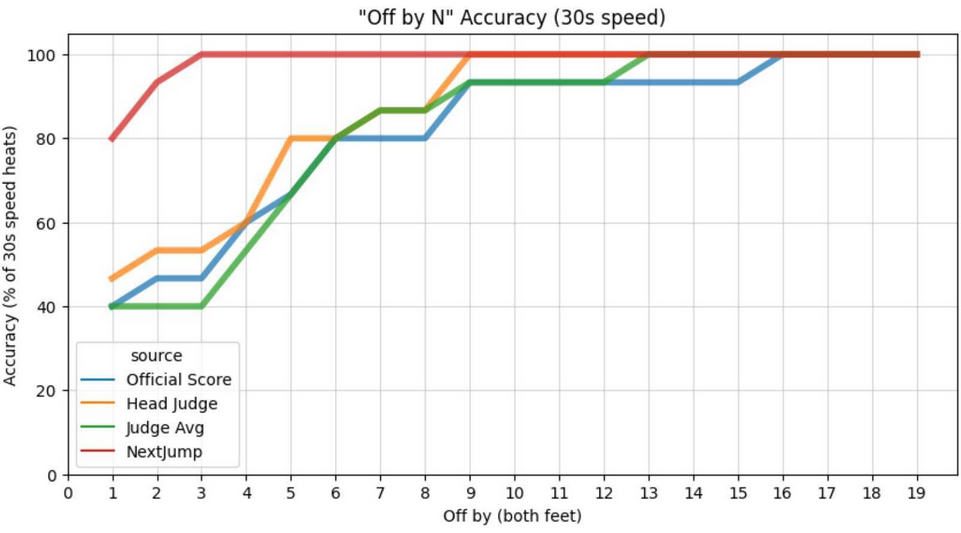
\includegraphics[width=0.95\linewidth]{img/nextjump-off-by-feet-judges}
    \caption[nextjump-results-multi]{Comparison of avg scores given to a jumper, compared to the effective score. Results are from 2024 AMJRF nationals. Provided by NextJump}
    \label{fig:nextjump-results-off-by-feet-judges-amjrf-2024}
\end{figure}

As of august 2023, \href{https://nextjump.app/}{NextJump} tested their AI-speed-counter, counting speed steps, on the world competition acquiring really accurate results, see fig \ref{fig:nextjump-results-off-by-feet-judges-amjrf-2024}.
The speed counter, counts how many (right-footed) times the speed step is performed. A speed step is the alternation between jumping left or right footed, like running but stationary. Between each alternation, a rope goes under your feet.
% TODO : add more information
They found that 10 hours was sufficient for a single event (e.g. just single rope speed) but to count all kinds of events more (diverse) data is needed. The current dataset entails 36h video material, including other events such as triples unders or double unders. Using this as a base/guidance, the likelihood to succeed implementing skill-recognition in freestyles grows.


\section{Human Action Recognition - general progress}

% TODO : find paper, reference to come to steps or use pareek again?
\textcite{Pareek_2020} summarized recent updates in human activity recognition. Based on their paper, a general approach is created in order to recognize the skills of jumpers.

As jumpers can stand everywhere in a field \footnote{A field is generally 12x12 or 15x15 meters}, locating and cropping athletes can improve the segmentation model \footnote{If time allows it, the final model can be compared with or without localization}. When the skippers are centered, action segmentation can be performed. This allows for the predicting of skills on newly recorded videos, without the need to cut out the different skills. Finally, a level can be mapped on each predicted skill \footnote{Note that in skillrecognition can infer turner involvements, number of rotations, hands, feet, ...}. Below you can find a summary of each step.

\begin{enumerate}
    \item Jumper localization
    \item Action segmentation, start/end of skill
    \item Skill prediction
    \begin{enumerate}
        \item Predict skill (power/gymnestic - pushup, split, cartwheel, ...)
        \item Predict turner involvement (cross, EB, TS)
        \item Predict number of rotations (single, double, triple, ...)
        \item Predict modifiers (1 hand, 2 feet, body rotations, ...)
    \end{enumerate}
    \item Level \& Score mapping
\end{enumerate}

In what follows, a study of past and recent advancements are listed for each of the three steps, localization, segmentation and prediction. This allows for a selection of machine learning models, best suited for the task at hand. After selecting potential models, some potential hurdles are listed which can withold progression on skill recognition.

\section{Jumper localization}
\label{subsec:jumper localization}

Image recognition has been at the centre of many recent studies. The best models mostly utilize Convolutional Neural Networks processing spacial information in the image \autocite{Zaidi_2021}. \textcite{Zaidi_2021} further compare recent models for object detection such as YOLO(v4), CenterNet, SSD, EfficientDet-D2, each using some backbone architecture like VGG-16, AlexNet, GoogleNet or lightweight models such as ShuffleNet or MobileNet (all using CNN's). A subset of these models being real-time models (fps > 30).
The goal of localizing the jumper is to center the athletes in the middle of the screen/video. \textcite{Bharadiya_2023} states that the position of objects in images doesn't really matter, but there are no clear statements about the size of objects. It could be that a jumper takes up 80 percent of the screen, while moments later he moved backwards and only takes up 30 percent of the video. The assumption is that centered and scaled data will work better later.

For the purposes of this study, it is possible to use one of the recent models of image recognition as a starting point, using transfer learning\footnote{Concept transfer learning explained in \autocite{Bharadiya_2023}} to fine-tune the results to localize the jumper.

To improve localization, video object segmentation or video instance segmentation can be used. VOS detects objects in videos, as compared to individual frames. \textcite{Gao_2022} lists some object segmentation models, like SwiftNet \autocite{Wang_2021} which uses ResNet18 as good and quick model.
Other possibilities would be Cutie \autocite{Cheng_2023}, DensePose (see fig \ref{fig:srwrap-bp}) \autocite{Guler_2018}

\begin{figure}
    \centering
    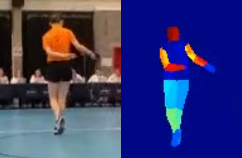
\includegraphics[width=0.3\linewidth]{../graphics/sr-denseposed}
    \caption[Image vs Densposed image]{Jumper in a routine wrapping the rope around her arm in a single rope routine. Image on the left is the original image, on the right is the simplified information after using detectron2 densepose \autocite{wu2019detectron2}}
    \label{fig:srwrap-bp}
\end{figure}

Densepose seems to be able to give the bounding boxes of the main poses detected. Perhaps just a convex hull and some padding will be enough for smart cropping and training a network from scratch is not needed.
However, a local tryout (without boxes) was rather slow, 1.2 fps on GPU within a Docker container.
As jumpers don't move that much most of the time, skipping some frames and smoothing out the prediction over the rest of the sequence or decreasing the amount of skipped frames when movement is detected can speed up the localization.

Even when Densepose isn't used, smoothing can still be applied to the guessed box as a video is basically a sequence of images.


\section{Video action segmentation}

When the athletes are cropped, videos need to be split \footnote{Not real/physical splits, but rather labels/annotations for where to split} in (sub)skills, because splitting new videos manually takes too much time and is impractical on competitions. A more specialized model like LTContext \autocite{Jiaming_2023} or a video vision model explored in section~\ref{subsec:bp-skill-recognition} could suffice.

Just like in localization, extracting poses, filtering foreground from background etc. could improve the segmentation.

The model for generating skill snapshots will
be useful for judging and subsequently labeling
data. Rather than replaying the video, judges can
just sequentially go through each trick one at a
time to assign, annotate or validate the predicted
skill.




\section{Skill recognition}
\label{subsec:bp-skill-recognition}

The final step would be to recognize the total skill in a freestyle video.
\textcite{Yin_2024} did a general HAR survey, mainly focused on team sports, in which they describe the evolution from normal CNN architectures, to recurrent neural networks for time sequences, remembering context, like the Long Short Term Memory model (LSTM), after which models were developed feeding the CNN output into LSTM or even implementing a convolutional filter in the memory cell \autocite{Shi_2015}.

\textcite{Wang_2019} investigated an improvement for current convolutional or recurrent models. They found that LSTM memory cells were too simple to contain higher-order complexities. As a result, they designed a memory in memory component, to replace the previous cell, which could predict actions on complexer data sets. This quickly formed the name Memory in Memory, MIM. Later, \textcite{Lin_2020} used a self-attention memory cell inside the convLSTM that can memorize global aspects in space and time. With about 35\% the number of parameters compared to Wang's MIM-model, SAM achieved a similar score as on the moving MNIST dataset, but faster. Although the focus of these papers was predicting future actions, the output can be transformed into a classification model, rather than a prediction model.

Another approach would be using transformers as a described  in \textcite{Yin_2024}. Options are the video vision transformer \autocite{Arnab2021} or adaptions like the ViT-TAD model by \textcite{Yang_2023}, Swin transformer \textcite{Liu_2021} or VideoMAE v2 by \textcite{Wang_2023}. Further research/try-outs will be required to ensure the transfer models can predict actions.

For reference, NextJump uses a CNN - MobileNetv4, \autocite{MobileNetv4_2024} and a transformer to analyze the full sequence and count. So using the convLSTM, SAM, MobileNet, or a transformer brings us to a better definition or example of what exactly we want to predict.

% TODO : SA_ConvLSTM?
% TODO : MViT

Even with a broad range of options, it isn't bad to think about potential hurdles. One of them are unknown of unusual skills. While a judge may refer to a head judge or think for itself, the AI model wouldn't be trained for that. The other hurdle could be that DD3 freestyles are a group activity, making it hard for models to recognize the required aspects. 

\section{Group activity}

As DD3 is a group activity, problems could arise while trying to detect skills. However, the hypothesis is that a DD3 freestyle always acts as one unit, thus not really requiring much special attention. One potential problem could be not know left from right, as there are two turners. Other problems might arise when adapting SR to SR2 where two individuals are not exactly one unit. Some further research can be done in models like stagNet \autocite{Qi_2020} to account for this idea. Another idea would be to apply the same method as YOLO, predicting multiple locations at the same time.




\section{Unknown/Unusual skills}
\label{subsec:bp-literature-unknowmultin-unusual-skills}

% TODO revise
Unknown skills or special cases pose another challenge. That's why the skill-matrix needs to defined in such a way, to accommodate for new combinations or skills. This is called zero-shot learning, \autocite{Pourpanah_2022}, where actions or combinations get recognized without any labels.

(Sort of marking unique skills as "I don't know" so that others new/unique ones will also be marked as "I don't know") Unusual skills on the other hand should be incorporated into the implementation.
A more concrete example would be turntables, which are mainly performed using a crab or push-up, but also seen with a frog or a split.
Turntables even have the potential to be combined with a swift. Omitting turntable frogs or splits in the train dataset can test this the ability to perform on unusual skills.




\section{Summary literature}
\label{subsec:bp-summary literature}

According to the state of the art, it appears feasible to analyze the performed skills in a given recording. In order to evaluate this, a proof of concept will be developed predicting jump rope skills. Sequentially, three steps are be required. The first step involves localizing the position of the athletes. This way, computational resources can be spared in the following steps, namely segmenting and recognizing. The segmentation consists of predicting split moments which should divide the video into likely skills. In the final step, the recognition step, each seperated skill can be analyzed by a vision model, predicting the most likely skill performed for the given section.

When all skills are predicted, corresponding levels and numeric scores can mapped onto each skillsection. These scores add up to difficulty score, usable to decide a victor on competitions.